\subsubsection{算法设计}

\paragraph{模型建立} 记报童每天购入报纸数量为$n$,需求量为$r$,服从正态分布$N(\mu, \sigma^2)$,其概率密度函数为$f$,批发价为$a=A(1-n/K)$,每份报纸的零售价为$b$,退回价为$c$,则报童每天的利润$V$为,
\begin{equation}\label{eq:ex7_profit}
    V(n)=\sum_{r=0}^{n-1}[(b-a) r-(a-c)(n-r)] f(r)+\sum_{r=n}^{\infty}[(b-a) n] f(r)
\end{equation}

其图像如\Cref{fig:ex7_profit},可以看到,随着购入报纸数量$n$的增大,利润$V$首先在$n=2000$附近出现了一个极大值,然后降低到负值,然而,随着$n$的继续增大,$V$的值出现了急速的攀升,甚至超过了之前的极大值。这是因为随着$n$的增大,批发价格$a$逐渐降低,当$n>15000$时,批发价格竟然低于回收价格,当$n>50000$时,批发价格甚至变成了负数,在这些情况下,报童只要多购进报纸,再统一进行回收,就能赚到差价,显然是不符合实际情况的。为了保证批发价与回收价之间有一定的差价,这里对$n$的范围做如下规定,
\begin{equation}
    0 \le n \le 5000
\end{equation}

\begin{figure}[H]
    \centering
    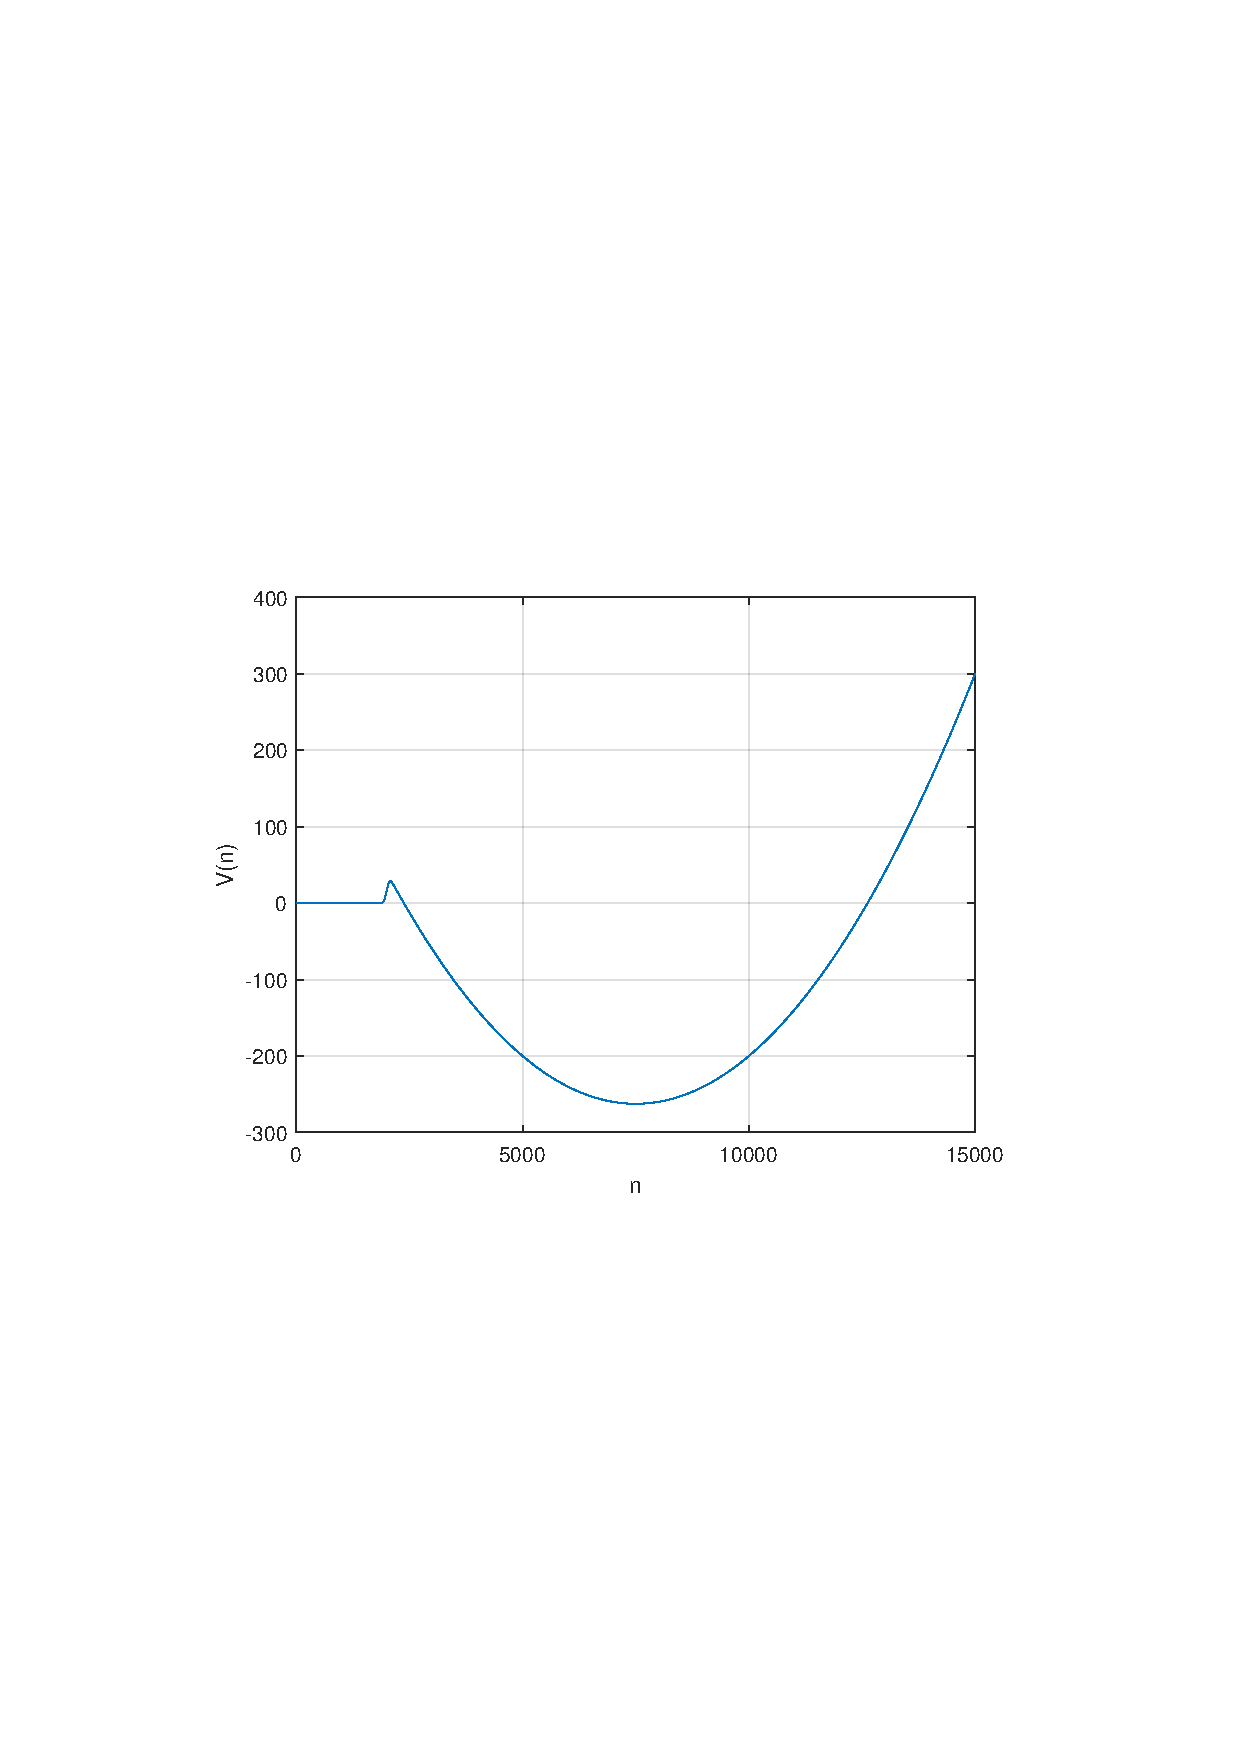
\includegraphics[width=0.8\textwidth,trim={3.09cm 9.295cm 3.09cm 9.295cm},clip]{fig/ex7_profit.pdf}
    \caption{利润$V$随购入报纸数量$n$变化的图像}
    \label{fig:ex7_profit}
\end{figure}

将$r$和$n$看作连续变量,则\Cref{eq:ex7_profit}可写作,
\begin{equation}
    V(n)=\int_0^n [(b-a) r-(a-c)(n-r)]f(r)dr + \int_n^{+\infty} (b-a)nf(r) dr
\end{equation}

注意这里$a$是关于$n$的函数,两边对$n$求导,化简得,
\begin{equation}
    V'(n) = \int_0^n \left(\frac{2An}{K}-A+c\right) f(r) dr + \int_n^{+\infty} \left(\frac{2An}{K}-A+b\right)f(r)dr
\end{equation}

令$V'(n)=0$,得到,
\begin{equation}
    \frac{\int_0^n f(r)dr}{\int_n^{+\infty} f(r)dr} = \frac{-2An+AK-bK}{2An-AK+cK}
\end{equation}

考虑到均值$\mu$比标准差$\sigma$大得多时,有$\int_0^n f(r)dr \approx \int_{-\infty}^n f(r)dr$,由对称性可知$\int_n^{+\infty} f(r)dr = 1-\int_{-\infty}^n f(r)dr$,因此得到,
\begin{equation}\label{eq:ex7_model}
    \int_{-\infty}^n f(r) dr = \frac{2An-AK+bK}{K(b-c)}
\end{equation}

\Cref{eq:ex7_model}即为本题的模型。

\paragraph{算法实现} \Cref{eq:ex7_model}是一个超越方程,无解析解,可采用\texttt{fzero}命令求解方程,采用\texttt{normcdf}命令计算正态分布的累积分布函数。

\subsubsection{程序}

请参见附录\ref{sec:ex7_code}。

\subsubsection{计算结果}

取初值为$n_0=2000$,计算得到最优购入报纸份数为$n=1968$。

\subsubsection{结果分析}

当限制$0 \le n \le 5000$时,批发价格$a$的取值范围为$0.45 \le a \le 0.5$,此时始终满足$c \le a \le b$,且批发价格与回收价格之间至少有0.1的差价,这是符合实际情况的。在这种限制下,求得的结果为全局最大值,可以作为实际应用的参考。

\subsubsection{结论}

为了获得最大利润,报童每天购进的报纸数应为1968份。
